\documentclass[12pt,a4paper,twoside]{article}
\usepackage{microtype}
\usepackage{graphicx}
\usepackage[utf8]{inputenc}
\usepackage{amsmath,amsfonts,amssymb}
\usepackage{subcaption}
\usepackage{float}
\usepackage{caption}
\usepackage{booktabs}
\usepackage{pgfplots}
\pgfplotsset{compat=1.18}
\usepackage{array}
\usepackage{multirow}
\usepackage{capt-of}
\usepackage{longtable}
\usepackage{tabularx}
\usepackage{wrapfig}
\usepackage{siunitx}
\usepackage{multicol}
\usepackage{listings}
\usepackage{qrcode}
\usepackage[T1]{fontenc}
\usepackage{mfirstuc}   
\usepackage{lipsum}    
\usepackage[most]{tcolorbox}
\usepackage{xcolor}
\definecolor{OxfordBlue}{HTML}{002147}
\definecolor{noteblue}{RGB}{0, 102, 204}
\definecolor{notebg}{RGB}{240, 245, 255}
\definecolor{darkred}{RGB}{139, 0, 0}
\definecolor{todo}{HTML}{e74c3c} 
\definecolor{tip}{HTML}{2ecc71} 
\definecolor{warning}{HTML}{f1c40f} 
\definecolor{note}{HTML}{3498db}   
\definecolor{darkburgundy}{RGB}{139, 0, 0} 

\usepackage[a4paper]{geometry}
\geometry{
  top=1in,
  bottom=1in,
  left=1.25in,
  right=1in
}

\usepackage{fancyhdr}
\pagestyle{fancy}
\renewcommand{\headrulewidth}{0pt}
\fancyhf{}

\fancyfoot[RO]{
    \footnotesize
    \textcolor{gray}{© 2025--2026 Maroua Mezhoud}
    \quad
    \textcolor{gray!60!black}{\rule[-0.5pt]{0.5pt}{8pt}}
    \quad
    \textcolor{black}{\thepage}
}

\fancyfoot[LE]{
    \footnotesize
    \textcolor{black}{\thepage}
    \quad
    \textcolor{gray!60!black}{\rule[-0.5pt]{0.5pt}{8pt}}
    \quad
    \textcolor{gray}{© 2025--2026 Maroua Mezhoud}
}

\newtcolorbox{mynotebox}{
    enhanced,
    breakable,
    colback=notebg,
    colframe=notebg, 
    borderline west={3pt}{0pt}{noteblue}, 
    arc=4pt,
    outer arc=4pt,
    left=15pt, 
    right=10pt,
    top=10pt,
    bottom=10pt,
    title=,
    fonttitle=\bfseries\sffamily,
    coltitle=noteblue,
    attach title to upper,
    after title={\\[0.5em]},
}

\newtcolorbox[auto counter,number within=section]{block}[1][]{
    enhanced jigsaw,
    coltitle=#1,                       
    colback=#1!08!white,               
    colframe=#1!08!white,              
    fonttitle=\bfseries\sffamily,       
    sharp corners=west,                
    detach title,                      
    borderline west={.85mm}{0pt}{#1},  
    pad at break=1mm,
    top=4mm,
    bottom=4mm,
    % Logic to rename 'todo' to 'To-Do' and capitalize others
    title={\ifstrequal{#1}{todo}{Interpretation of Results}{\capitalisewords{#1}}},
    % Adds spacing between the title and the content
    code={\ifdefempty{\tcbtitletext}{}{\tcbset{before upper={\tcbtitle\par\medskip}}}},
}


\usepackage{hyperref}
\hypersetup{
    colorlinks=true,
    linkcolor=black,
    urlcolor=OxfordBlue
    }

\usepackage{wallpaper}

\usepackage{background}
\backgroundsetup{
  scale=4,
  color=gray!50,
  opacity=0.2,
  angle=55,
  contents={}  
}

\usepackage{eso-pic}


\usepackage{listings}
\usepackage{xcolor}

\definecolor{codegray}{rgb}{0.45,0.45,0.45}
\definecolor{codebackground}{rgb}{0.98,0.98,0.97} % أبيض مائل للدفء الخفيف
\definecolor{keywordcolor}{rgb}{0.20,0.35,0.60}   % أزرق أكاديمي داكن
\definecolor{commentcolor}{rgb}{0.65,0.40,0.55}   % وردي أكاديمي هادئ
\definecolor{stringcolor}{rgb}{0.60,0.20,0.70}    % بنفسجي أقوى وواضح

\lstset{
    language=Python,
    basicstyle=\ttfamily\small,     
    backgroundcolor=\color{codebackground},
    keywordstyle=\color{keywordcolor}\bfseries,
    commentstyle=\color{commentcolor}\itshape,
    stringstyle=\color{stringcolor},
    numbers=left,
    numberstyle=\tiny\color{codegray},
    stepnumber=1,
    numbersep=10pt,
    frame=single,            
    framerule=0.5pt,
    rulecolor=\color{gray!30},
    breaklines=true,
    showstringspaces=false,
    tabsize=4,
    captionpos=b,
    xleftmargin=15pt
}


\begin{document} %===============================================

\begin{titlepage}

\ThisCenterWallPaper{1}{images/Front-Page-BG.pdf}

\centering

\begin{flushleft}
    
\includegraphics[width=0.18\textwidth]{images/footer-logo.png}
\end{flushleft}


\vspace{1cm}

{\Large \textbf{Mohamed El Bachir El Ibrahimi University of Bordj Bou Arréridj} \par}

{\large Faculty of Science and Technology \par}

{\large Department of Materials Science \par}

{\large Undergraduate Programme (LMD) - Physics – Year 2\par}
   
{\large Course: Thermodynamics \par}
   
\vspace*{\fill}
{\Huge \textbf{Practical Work  N\textsuperscript{o}:4} \\ \textbf{Thermal Conductivity in Construction Materials } \par}
{\large \textbf{According to the plate method with Cassy}\par}

 
\vspace*{\fill}

  {\large \textbf{Submitted by:} \\ Maroua Mezhoud \par}
  {\large \par}

\vspace{1 cm}
    
    {\large \textbf{Supervised by:} \\ Dr. N. Benchiheub\par}
    { Group: 2\par}
    
\vspace{2 cm}

    {\large Date of submission: \today \par}
   
    {\large Academic Year: 2025–2026 \par}  

\vfill
    
\end{titlepage}

\pagenumbering{Roman}  
\pagestyle{plain}


\begin{abstract}

\textit{This report investigates heat conduction in three different construction materials (\textbf{Wood, Fermacell, and Rohacell}) using the plate method with the Cassy system. The thermal conductivity is determined from measurements of electrical power and temperature difference across the samples. The experimental results are compared with literature values in order to assess their accuracy and discuss possible sources of error. In addition, a Python-based simulation is used to illustrate the temporal evolution of temperature and its consistency with Fourier’s law. An open-source repository is provided to ensure transparency and reproducibility.}

\end{abstract}

\tableofcontents

\listoffigures

\listoftables

\newpage 

\pagestyle{fancy} 

\pagenumbering{arabic}
\setcounter{page}{1}    



\section{Introduction}

Heat conduction is a fundamental mode of heat transfer in thermodynamics, occurring within materials due to temperature gradients without any macroscopic motion of matter. This process is governed by Fourier’s law and is characterized by the thermal conductivity, an intrinsic property that depends on the nature and structure of the material.

In the field of construction, thermal conductivity is a key parameter for evaluating the thermal performance of materials, as it determines their ability to either conduct or resist heat transfer. This property plays a crucial role in energy efficiency and thermal insulation in buildings.


\section{Objectives}
\begin{itemize}
    \item Graphical representation of the temperature evolution of different material samples over time.
    \item Qualitative observation of the establishment of thermal equilibrium.
    \item Determination of thermal conductivity $\lambda$ of samples of certain building materials from the temperature difference $\Delta T$.
\end{itemize}

\section{Theoretical Background}




Thermal conductivity or conductibility $\lambda$ (lambda), expressed in units $W/m.K$ is a physical quantity that designates the capacity of materials to transmit heat in a solid medium by conduction without macroscopic movement of matter. The conductivity coefficient is involved in the law named after the French physician Fourier. When the material is homogeneous and isotropic, Fourier's law is written as:

\begin{equation}
\vec{J} = -\lambda \vec{grad} T
\end{equation}

Here $\vec{J}$ is the heat flow density measured in $W/m^2$ \\
$\vec{grad} T$ temperature gradient, is written as a function of the partial derivatives by:

\begin{equation}
\vec{grad} T = \vec{\nabla} T = \left( \frac{\partial T}{\partial x} \vec{i} + \frac{\partial T}{\partial y} \vec{j} + \frac{\partial T}{\partial z} \vec{k} \right)
\end{equation}

Thermal conductivity is an intrinsic constant characteristic of each material. It is valid for bodies with homogeneous surfaces and can vary depending on:

\begin{itemize}
    \item The material's temperature,
    \item Its humidity level,
    \item And its density.
\end{itemize}

The higher conductivity coefficient $\lambda$, the more the material conducts heat; however, a low coefficient is considered an insulator. Insulating materials often have $\lambda$ values between 0.025 and 0.050 $W/m.K$, including wood, clay, etc.

In this experiment, we will study the thermal conductivity of building materials in the form of a plate of thickness $d$ and surface area $S$. Both surfaces are maintained at temperatures $T_1$ and $T_2$. For example, we consider $T_2 > T_1$.


\begin{figure}[htbp]
    \centering
    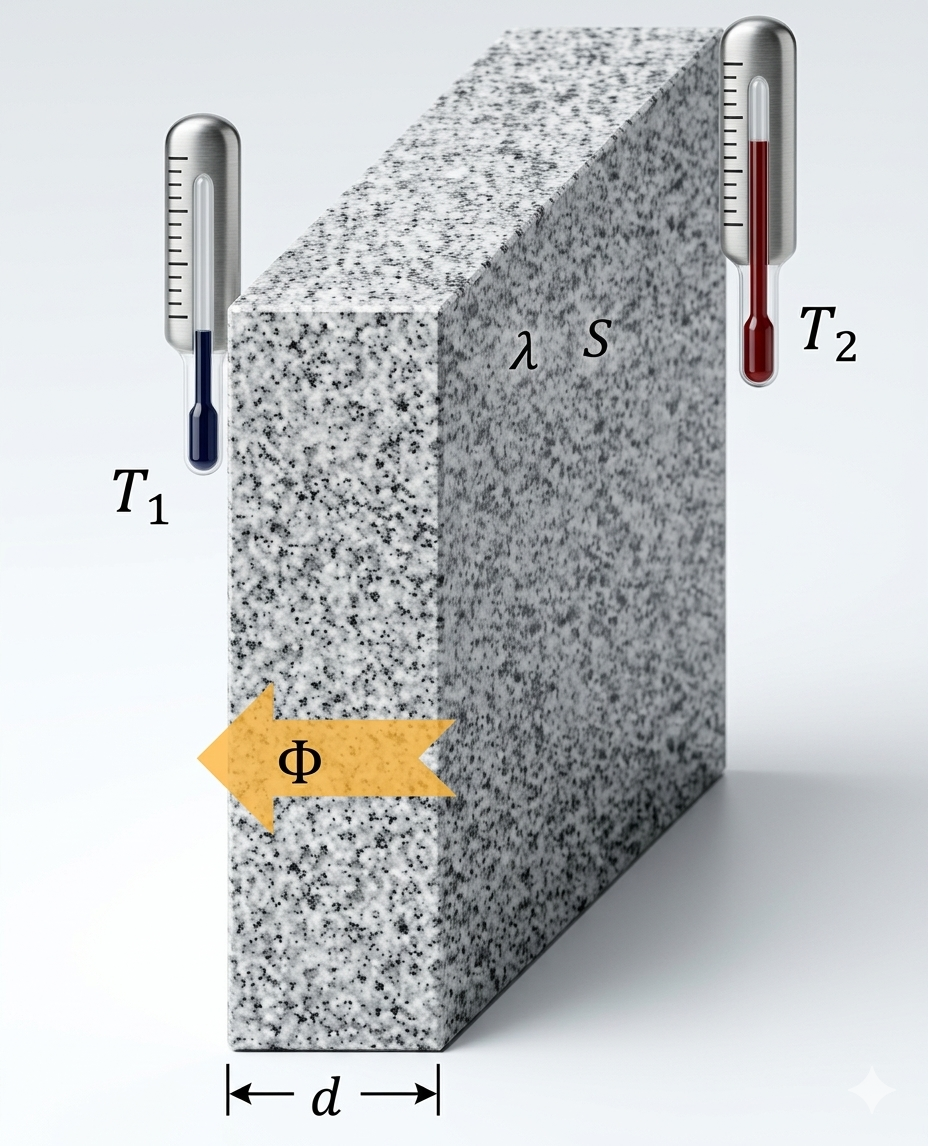
\includegraphics[width=0.4\textwidth]{images/Gemini_Generated_Image_2xwgy42xwgy42xwg.png}
    \caption{Heat conduction through a solid with thickness $d$ and conductivity $\lambda$.}
    \label{fig:heat_conduction}
\end{figure}


Then the heat flow transferred between the two walls of the plate is expressed with respect to the thermal conductivity by the following relation:

\begin{equation}
\phi = \frac{\Delta Q}{\Delta t} = \lambda \frac{S}{d} \Delta T
\end{equation}

With $\Delta T = (T_2 - T_1)$ gradient temperature.

From which, the thermal conductivity can be easily calculated by a direct measurement of the temperature difference $\Delta T$ and the transferred heat flux according to the relation:

\begin{equation}
\lambda = \frac{\frac{\Delta Q}{\Delta t} \cdot d}{S} \frac{1}{\Delta T}
\end{equation}

To measure heat flow, a heat-insulated enclosure is used in the calorimeter chamber, which ensures uniform heat flow through the material and eliminates any heat loss. To create the heat flow through the material sample, the interior of the chamber is electrically heated. Outside, ice is placed directly on the sample. When thermal equilibrium is reached, i.e., in a steady state where the temperature is constant over time at all points, the electrical power $P$ corresponds exactly to the heat flow $\phi$, so it becomes

\begin{equation}
\frac{\Delta Q}{\Delta t} = P
\end{equation}

Or else

\begin{equation}
P \cdot t = W = Q
\end{equation}

means that, the work provided $W$ is equal to the thermal energy which passes through the plate of material. The thermal conductivity is then given as a function of the electrical power such that:

\begin{equation}
\lambda = P \frac{d}{S} \frac{1}{\Delta T}
\end{equation}

To obtain the temperature difference at thermal equilibrium, the below experimental steps must be followed:

\begin{itemize}
    \item Measure the temperature $T_i$ of the lower surface (below) of the material plate, corresponding to the interior of the chamber.
    \item Measure the temperature $T_e$ of the outer surface (above) of the ice-covered material plate.
    \item Record the temperature changes over time, over a long period (approximately 1 hour).
\end{itemize}

The temporal variation of the internal temperature is proportional to this temperature, with the addition of a constant such as:

\begin{equation}
\frac{\Delta T}{\Delta t} = aT + b
\end{equation}

Solving this equation leads to the expression of temperature as a function of time $T(t)$:

\begin{equation}
T(t) = T_{\text{éq}_{\text{int}}} - T_{\text{diff}} e^{-\frac{t}{\tau}}
\end{equation}

where: $T_{\text{éq}_{\text{int}}}$ internal equilibrium temperature.  
$T_{\text{diff}} = (T_{\text{éq}_{\text{int}}} - T_i)$ temperature difference.

And $\tau$ time constant.

Since the above equation is identified with a function of the form:

\begin{equation}
T(t) = A - B e^{\left(\frac{-x}{C}\right)}
\end{equation}

The thermal equilibrium temperature of the heated face of the building material results from the identification of this function with the values recorded in the experiment. Where the parameter $A$ obtained corresponds to the desired internal equilibrium temperature $T_{\text{éq}_{\text{int}}}$.

However, the external temperature of the upper face of the material plate is kept low (constant) thanks to the ice, and since slight variations in the external temperature can still occur, using the average value of the external temperature values $T_{\text{froid}}$, we can easily find the temperature difference $\Delta T$ by:

\begin{equation}
\Delta T = T_{\text{éq}_{\text{int}}} - T_{\text{froid}}
\end{equation}

And therefore, it will be simple to experimentally determine the thermal conduction coefficient $\lambda$ of building materials according to the relation (8).


\section{Apparatus and Materials}

To carry out the setup of the experiment represented by the figure below, we will use the following elements:

\begin{itemize}

    \item \textbf{Calorimetric chamber}:
    \begin{itemize}
        \item Heat-insulated enclosure (1) made of thermally insulating materials with a square opening (3) in the middle (see figure 2), through which plates of material to be tested are introduced, and which is covered with foam rubber.
        
        \item The air temperature in the chamber is measured by inserting the thermometer or probe through the channel (2) with three rubber stoppers (13), two of which are pierced with different diameters while the other is not pierced.
        
        \item The chamber is equipped with three channels (4) for measuring the temperature of the building materials inside the chamber and on the inner and outer faces of the samples.
        
        \item Two pairs of sockets:
        \begin{itemize}
            \item (5) for threading the plate heater (7)
            \item (6), electrically connected to (5), used to power the plate heater
        \end{itemize}
        
        \item A mounting hook (8)\footnote{\textbf{The mounting hook (8)} was replaced by a random screwdriver I keep in my bag for no reason}.
        
        \item A set of plates of building materials: ceramic, polystyrene, aluminum, plexiglass. Dimension $15\text{cm} \times 15\text{cm}$ with two grooves (10) for inserting the probes, and at the end of each groove a recess (11) for placing the contact pads.
    \end{itemize}

    \item A soft plastic serrated spatula \textbf{(12)}

    \item A transformer \textbf{(14)} ($2 \dots 12\text{ V}, 120\text{ W}$) delivering alternating voltages


\item 
\begin{minipage}[t]{0.6\textwidth} 
    A detector Sensor-CASSY 2 (15) cascade-connectable interface for data acquisition. This device is essential for real-time measurements and allows for multi-channel data logging and digital processing of physical quantities.
\end{minipage}
\hfill
\begin{minipage}[t]{0.3\textwidth} 
    \vspace{-1.5cm}
    \centering
    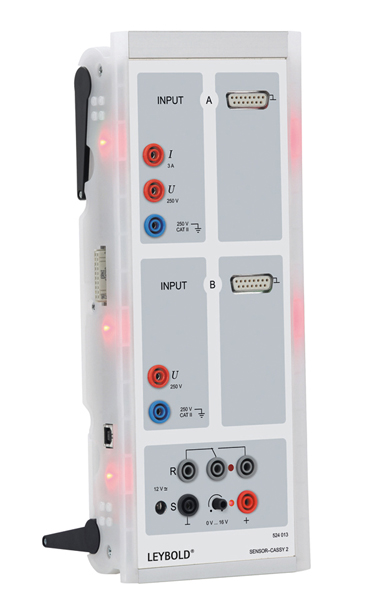
\includegraphics[width=\textwidth]{images/sensor cassy 2.jpg}
    \captionof{figure}{Sensor-CASSY 2}
    \label{fig:sensor_cassy_2}
\end{minipage}

    \item \textbf{Cassy Lab2}

    \item Temperature probe \textbf{NiCr-Ni (16)}:
    \begin{itemize}
        \item A type K thermocouple with standardized flat plug for use with CASSY and the adapter connector for the probe
    \end{itemize}

    \item Connection wires

    \item Ice \textbf{(17)}

    \item Thin plastic sheet

    \item A PC

    \item A tube of conductive paste

\end{itemize}



\begin{figure}[htbp]
     \centering
     \begin{subfigure}[b]{0.45\textwidth}
         \centering
         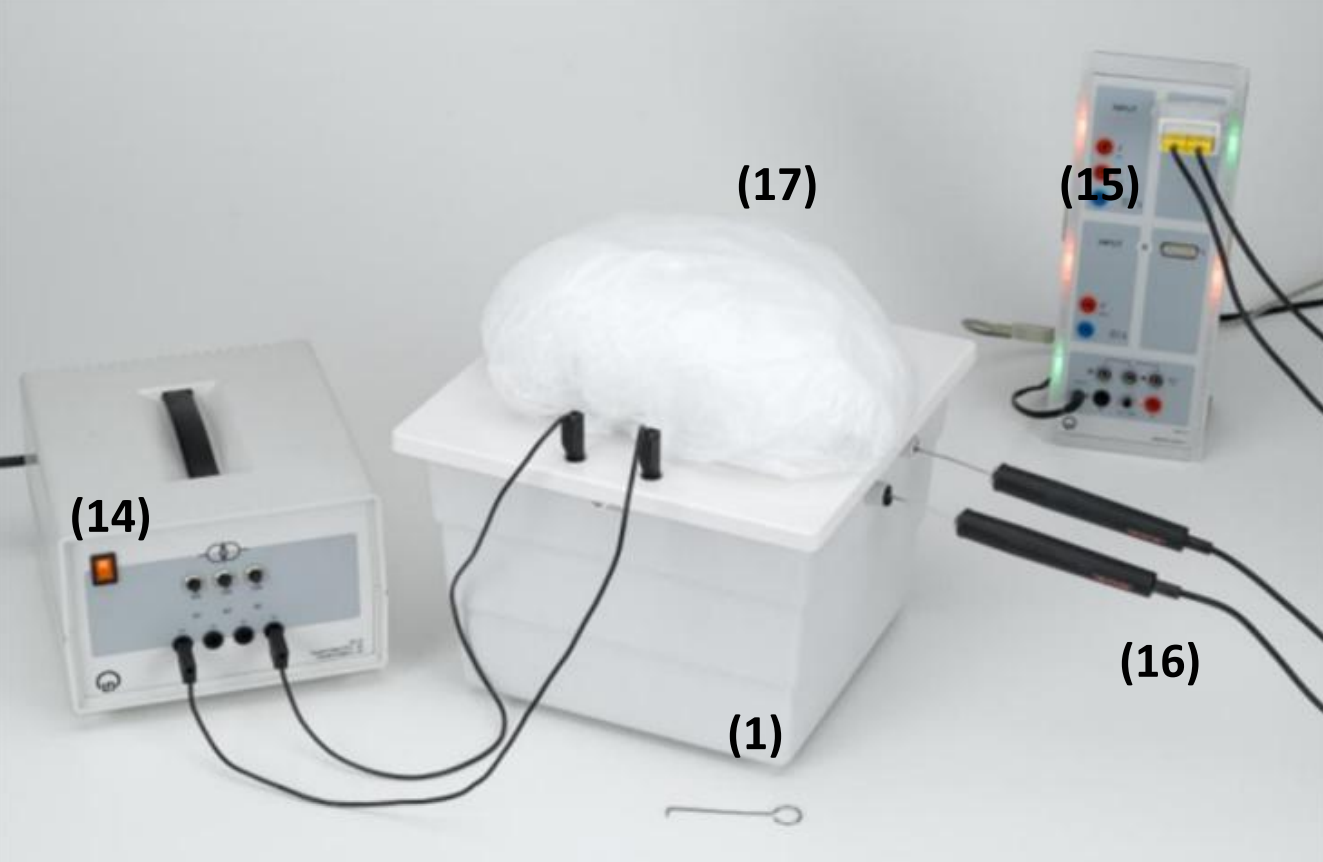
\includegraphics[width=\textwidth]{images/Screenshot 2026-03-16 154304.png}
         \caption{Assembly of the experiment}
         \label{fig:assembly}
     \end{subfigure}
     \hfill
     \begin{subfigure}[b]{0.45\textwidth}
         \centering
         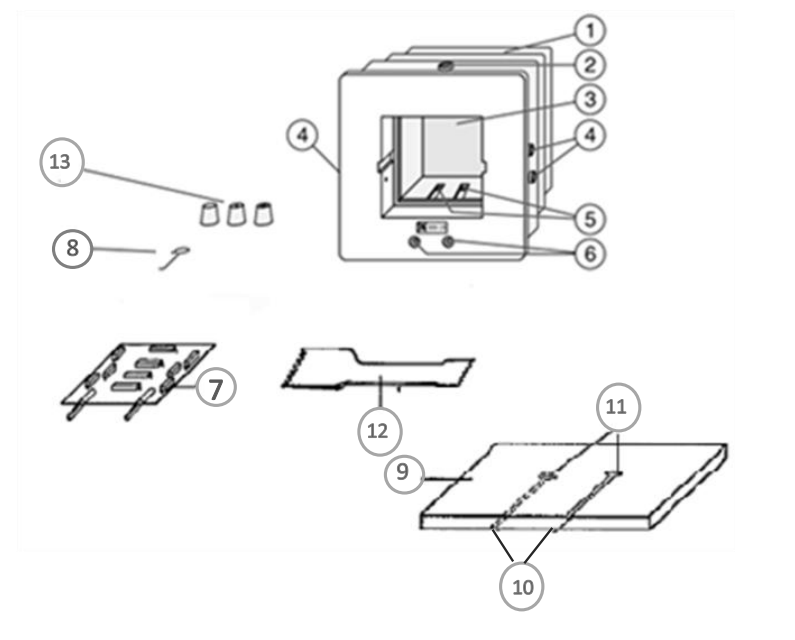
\includegraphics[width=\textwidth]{images/Screenshot 2026-03-16 154537.png}
         \caption{Heat chamber with accessories}
         \label{fig:heatchamber}
     \end{subfigure}
     
     \caption{Experimental setup and components}
     \label{fig:total_setup}
\end{figure}

\begin{block}[warning]
Do not exceed the heating temperature \textbf{$60^{\circ}C$} of the calorimetric chamber and the construction materials.
\end{block}


\section{Experimental realization}

It is necessary to determine the power of the plate heater before starting the experiment. To do this, the calorimetric chamber must be put into operation without any material plates.

\subsection*{a- Power measure $P$}

\begin{itemize}
    \item Ensure that the transformer is disconnected, then connect the transformer and the chamber to the Sensor-Cassy according to the assembly illustrated in the figure below in order to measure the voltage and current.
\end{itemize}

\begin{figure}[H]
    \centering
    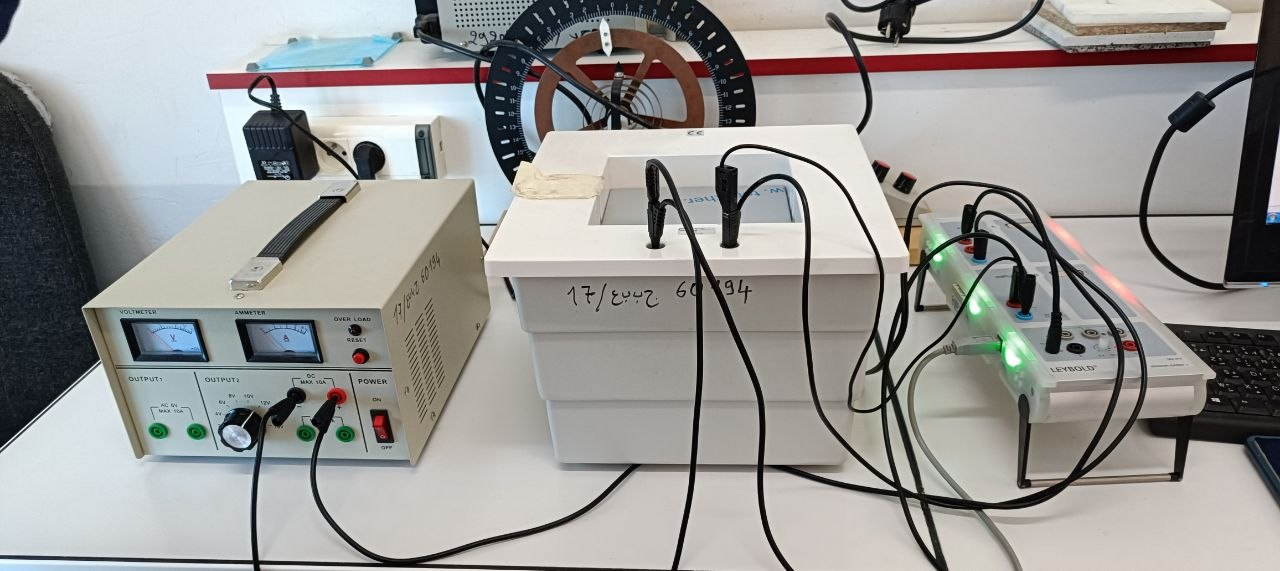
\includegraphics[width=1\textwidth]{images/montage.jpg}
    \caption{Experimental setup for determining heating power}
    \label{}
\end{figure}

\begin{itemize}
    \item Load settings into Cassy Lab 2.
\end{itemize}

Turn on the transformer, observe the voltage $U_{B1}$ and the intensity of the current $I_{A1}$, record the values obtained. Note the power $P$

\begin{itemize}
    \item Stop the transformer.
\end{itemize}

\begin{block}[warning]
item The transformer must remain in service for the shortest time to carry out this measurement. Then, wait for the plate heater to cool completely to room temperature.
\end{block}

\subsection*{b- Temperature measure}

\textbf{Material Plate Preparation and Assembly}

\begin{itemize}
    \item Place an aluminum contact pad in the circular sink on the selected material plate. Position it so that the hole is aligned with the groove. The pad establishes good thermal contact with the aluminum plates; they have a thermal conductivity 1000 times higher than that of the material samples.
    
    \item Apply thermal paste to the pad, then place a thin aluminum plate on the coated surface of the plate so that the black side is facing outward.
    
    \item Repeat the process with the other side. Press the plates together.
\end{itemize}

\textbf{Temperature Measurement Setup}

\begin{itemize}
    \item First, insert the tips of the temperature probes into the holes in the plugs (be careful not to deform them).
    
    \item Now place the prepared sample plate in the calorimeter chamber. Insert the temperature probes, one for each side. - Connect the temperature probes to the cassy sensor using the NiCr-NiS adapter.
    
    \item Connect the chamber to the transformer as shown in Figure 5.
\end{itemize}

\textbf{Cooling}

\begin{itemize}
    \item Spread a thin plastic sheet over the chamber, then place a sufficiently large thin bag filled with ice on the top of aluminum plate so that the ice bag has the best possible contact with the aluminum plate.
\end{itemize}


\begin{block}[warning]
\begin{itemize}
    \item Make sure that there is no water infiltration into the room or on the cables.
    \item Do not put the heat-conducting paste in the grooves.
\end{itemize}
\end{block}



\begin{figure}[H]
    \centering
    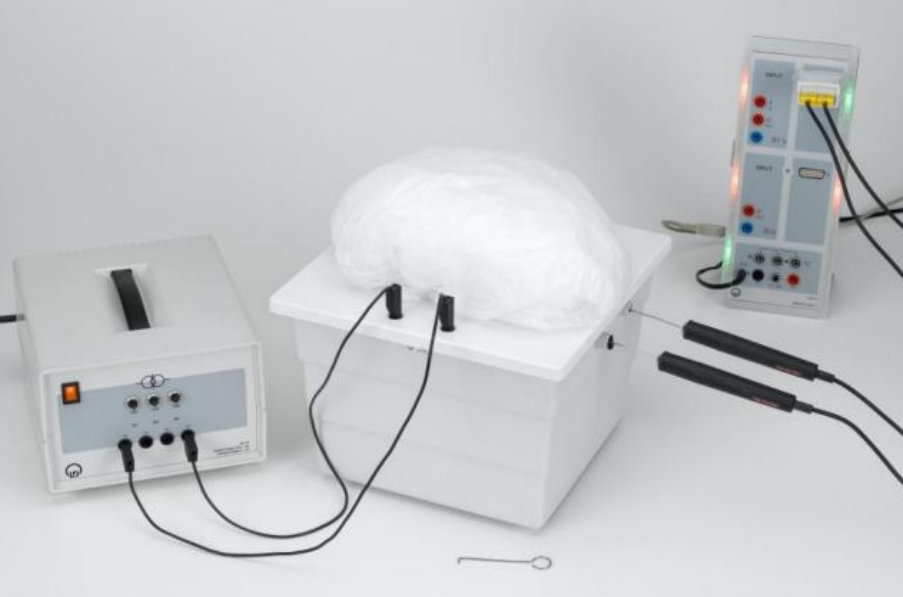
\includegraphics[width=1\textwidth]{images/Screenshot 2026-03-18 160319.png}
    \caption{Assembly for temperature measurement}
    \label{}
\end{figure}



\textbf{Measures realization}

\begin{itemize}
    \item Load the measurement parameters into Cassy Lab2 $\vartheta_{A11}$ et $\vartheta_{A12}$
    
    \item Turn on the transformer, wait to start the measurements;
    
    \item Observe both temperatures and wait until the higher temperature begins to rise.
    
    \item In this case, start the measurement, plotting the temperature variation over time.
    
    \item As soon as the measurements are complete, stop the measurements and then the transformer.
    
    \item Remove the temperature probes, then remove the building material using the mounting hook.
\end{itemize}


\begin{block}[warning]
\begin{itemize}
    \item If the indoor temperature reaches 60°C, turn off the transformer and repeat the measurement with a lower voltage.
    \item Do not exceed the voltage of 6V for Rohacell foam board.
\end{itemize}
\end{block}


\section{Results and Discussion}




\begin{table}[H]
\centering
\renewcommand{\arraystretch}{1.5}

\begin{tabularx}{\textwidth}{>{\raggedright\arraybackslash}X *{3}{>{\centering\arraybackslash}X}}
\toprule
\textbf{Parameter} & \textbf{Material 1} & \textbf{Material 2} & \textbf{Material 3} \\
\midrule

Material nature 
& Wood 
& Fermacell 
& Rohacell \\

\multirow{1}{*}{Surface area $S\ (\si{m^2})$} 
& \multicolumn{3}{c}{$15^2 \times 10^{-4}$} \\

\multirow{1}{*}{Thickness $d\ (\si{m})$} 
& \multicolumn{3}{c}{0.01} \\

Work voltage $U\ (\si{V})$ 
& 10.23 
& 10.23 
& 5.52 \\

Current $I\ (\si{A})$ 
& 1.02
& 1.02
& 0.828 \\

Power $P\ (\si{W})$ 
& 10.435 
& 10.435 
& 4.267 \\

$T_{\text{eq,int}}\ (\si{\degreeCelsius})$ 
& 53 
& 48
& 40 \\

$T_{\text{froid}}\ (\si{\degreeCelsius})$ 
& 0 
& 0 
& 0 \\

$\Delta T\ (\si{K})$ 
& 53 
& 48
& 40 \\

Experimental conductivity $\lambda_{\text{exp}}\ (\si{W.m^{-1}.K^{-1}})$ 
& 0.087 
& 0.096
& 0.047 \\

Literature conductivity $\lambda_{\text{lit}}\ (\si{W.m^{-1}.K^{-1}})$ 
& 0.07 -- 0.17 
& 0.25 -- 0.35
& 0.03 -- 0.05 \\

\bottomrule
\end{tabularx}



\caption{Experimental results for thermal conductivity measurement}
\end{table}




\subsection*{Relative Error Analysis}

In order to evaluate the accuracy of the experimental results, the relative error between the experimental and literature values of thermal conductivity is calculated using the following expression:

\begin{equation}
\varepsilon = \frac{\left| \lambda_{\text{exp}} - \lambda_{\text{lit}} \right|}{\lambda_{\text{lit}}}
\end{equation}

For comparison, the average value of each literature range is considered.

\textbf{Wood:}

For wood, taking $\lambda_{\text{lit}} = 0.12\ \si{\watt\per\meter\per\kelvin}$:
\[
\varepsilon_{\text{wood}} = \frac{|0.087 - 0.12|}{0.12} = 0.275 \approx 27.5\%
\]

\textbf{Fermacell:}

For Fermacell, taking $\lambda_{\text{lit}} = 0.30\ \si{\watt\per\meter\per\kelvin}$:
\[
\varepsilon_{\text{Fermacell}} = \frac{|0.096 - 0.30|}{0.30} = 0.68 \approx 68\%
\]

\textbf{Rohacell:}

For Rohacell, taking $\lambda_{\text{lit}} = 0.04\ \si{\watt\per\meter\per\kelvin}$:
\[
\varepsilon_{\text{Rohacell}} = \frac{|0.047 - 0.04|}{0.04} = 0.175 \approx 17.5\%
\]



\begin{block}[todo]
It is important to note that the experimental value for\textit{ Rohacell} lies within the literature range, indicating a physically acceptable result despite the calculated relative error.

The results indicate that \textbf{Rohacell} presents the best agreement with literature values, followed by \textbf{wood} with a moderate deviation. In contrast, the \textbf{Fermacell} result shows a significant discrepancy, confirming that this measurement is unreliable.
\end{block}


\section{Conclusion and Sources of Error}

The experimental results lacked perfect accuracy due to the following reasons:

\begin{itemize}
    \item \textbf{Temperature Assumption:} Calculations were conducted assuming the ice temperature was $0^{\circ}\text{C}$. However, the actual recorded temperature was $19^{\circ}\text{C}$ because the ice was not fully frozen. We used $0^{\circ}\text{C}$ in our calculations to maintain a standardized baseline.
    
    \item \textbf{Time and Equipment Constraints:} We could not wait the required 10 minutes for the temperature to stabilize. This was necessary to prevent the device from exceeding the $60^{\circ}\text{C}$ threshold, as the temperature had already reached $40^{\circ}\text{C}$ and time was limited.
    
    \item \textbf{Data Reliability (Fermacell):} It is important to note that the experimental result for \textbf{Fermacell} \textcolor{darkburgundy}{was provided by the other group in our session, not calculated by our own group}. This specific result was found to be \textbf{highly inaccurate} and fell significantly outside the expected literature range. This discrepancy suggests potential procedural or measurement errors in their specific experimental run.
\end{itemize}

\subsection*{Comparison of Literature Thermal Conductivity Values}

Based on the literature conductivity values ($\lambda_{\text{lit}}$) reported in the study, the tested materials can be ranked in ascending order of thermal conductivity as follows:

\begin{itemize}
    \item \textbf{Rohacell:} This material exhibits the lowest thermal conductivity in the group, making it the best thermal insulator. Its conductivity ranges between $0.03$ and $0.05 \text{ W m}^{-1} \text{ K}^{-1}$.
    
    \item \textbf{Wood:} Wood has a moderate thermal conductivity compared to Rohacell, with values ranging from $0.07$ to $0.17 \text{ W m}^{-1} \text{ K}^{-1}$.
    
    \item \textbf{Fermacell:} This material shows higher thermal conductivity, ranging between $0.23$ and $0.38 \text{ W m}^{-1} \text{ K}^{-1}$.
\end{itemize}



\section{Numerical Simulation and Theoretical Modeling}

Due to the storage unit's exposure to a digital virus that led to the corruption of the raw data, a numerical simulation was conducted using Python based on the mathematical model
\[
T(t) = A - B e^{-t/C}
\]
This was performed using the theoretical values of the material in order to demonstrate the expected thermal curve behavior and its consistency with Fourier’s law of heat conduction.

\subsection{Numerical Simulation Code}


\begin{lstlisting}[language=Python]

import numpy as np
import matplotlib.pyplot as plt

# 1. Mathematical Model (Exponential Heating Model)
# T(t) represents the temperature increase over time towards steady state
def thermal_model(t, A, B, C):
    return A - B * np.exp(-t / C)

# 2. Experimental Parameters (Extracted from Rohacell data table)
d = 0.01                # Material thickness in meters (1 cm)
S = 15**2 * 1e-4        # Surface area in square meters (0.0225 m^2)
P = 4.267               # Electrical power input in Watts (U * I)
T_eqint = 40.0          # Measured steady-state temperature (Asymptote A)
T_froid = 0.0           # Cold plate temperature (Ice reference)

# Verification of Experimental Thermal Conductivity (Lambda)
# Formula: lambda = (P * d) / (S * Delta_T)
lambda_exp = (P * d) / (S * (T_eqint - T_froid))

# 3. Curve Fitting Parameters for Simulation
A = T_eqint             # Horizontal asymptote (Final equilibrium temperature)
B = A - 20              # Temperature difference (Assumes initial T = 20°C)
C = 650                 # Time constant (Determines the curve's slope)

# 4. Synthetic Data Generation
# Simulating 1 hour of data collection (3600 seconds)
t_data = np.linspace(0, 3600, 250)  
# Adding Gaussian noise to mimic real Cassy sensor fluctuations
noise = np.random.normal(0, 0.15, t_data.shape) 
T_data = thermal_model(t_data, A, B, C) + noise

# 5. Professional Visualization
plt.figure(figsize=(11, 6))

# Plotting simulated data points
plt.scatter(t_data, T_data, color='gray', s=10, alpha=0.4, label='Reconstructed Cassy Data (Rohacell)')

# Plotting the optimized theoretical fit
plt.plot(t_data, thermal_model(t_data, A, B, C), color='#2E86C1', linewidth=2.5, label='Theoretical Fit')

# Graphical enhancements for report quality
plt.axhline(y=A, color='red', linestyle='--', alpha=0.7, label=f'Equilibrium Temp (A) = {A}°C')
plt.title('Thermal Conductivity Analysis: Rohacell Simulation', fontsize=14, pad=20)
plt.xlabel('Time $t$ (seconds)', fontsize=12)
plt.ylabel('Temperature $T$ (°C)', fontsize=12)

# Displaying the calculated Lambda on the plot
plt.text(2000, 25, f'$\lambda_{{exp}} = {lambda_exp:.4f} \ W/(m\cdot K)$', 
         fontsize=12, bbox=dict(facecolor='white', alpha=0.5))

plt.legend(loc='lower right')
plt.grid(True, which='both', linestyle='--', alpha=0.5)
plt.tight_layout()

# Saving the figure in high resolution (300 DPI) for the final report
plt.savefig('Rohacell_Simulation.png', dpi=300)
plt.show()

\end{lstlisting}







\subsection{Simulation Results}

\begin{figure}[H]
    \centering
    
\includegraphics[width=1\textwidth]{images/that thing.png}
    \caption{Assembly for temperature measurement}
    \label{}
\end{figure}



\section{Source Code and Reproducibility}


\begin{mynotebox}
\begin{center}
    \begin{minipage}{0.7\textwidth}
        \centering
         In alignment with this principle, \textcolor{darkred}{all source code, simulation data, and figures associated with this work} are publicly available to ensure transparency and reproducibility.\\
        \href{https://github.com/Maroua-Mezhoud/Physics-Lab-Reports/tree/main/Thermodynamics-Lab-Reports}{\texttt{github.com/Maroua-Mezhoud}}
    \end{minipage}
    \begin{minipage}{0.2\textwidth}
        \centering
        \qrcode[height=2 cm]{https://github.com/Maroua-Mezhoud/Physics-Lab-Reports/tree/main/Thermodynamics-Lab-Reports}
    \end{minipage}
    \\ \vspace{1 mm}
    \footnotesize \textit{Scan or click to access the repository}
\end{center}
\end{mynotebox}






\newpage
\thispagestyle{empty}
\backgroundsetup{contents={© 2025--2026 Maroua Mezhoud}}
\BgThispage
\null

\newpage



\end{document}



